\documentclass[11pt,a4paper]{article}
\usepackage[utf8]{inputenc}
\usepackage[vietnamese]{babel}
\usepackage{amsmath,amssymb}
\usepackage[version=4]{mhchem}
\usepackage{geometry}
\geometry{top=0.65cm,bottom=0.65cm,left=1.25cm,right=1.25cm,headheight=20pt,headsep=3pt,footskip=9pt}
\usepackage{graphicx}
\usepackage{xcolor}
\usepackage{tabularx}
\usepackage{array}
\usepackage{tikz}
\usepackage{multicol}
\usepackage{fancyhdr}
\usepackage{enumitem}

\definecolor{hfRed}{HTML}{D32F2F}
\definecolor{hfGreen}{HTML}{8BC390}
\definecolor{mainGreen}{HTML}{2E7D32}

\usepackage{ex_test}

\pagestyle{fancy}
\fancyhf{}
\renewcommand{\headrulewidth}{0.75pt}
\renewcommand{\headrule}{\hbox to\headwidth{\color{hfGreen}\leaders\hrule height \headrulewidth\hfill}}
\renewcommand{\footrulewidth}{0.75pt}
\renewcommand{\footrule}{\hbox to\headwidth{\color{hfGreen}\leaders\hrule height \footrulewidth\hfill}}

\fancyhead[L]{\small\itshape\color{hfRed}Tài liệu lưu hành nội bộ}
\fancyhead[R]{\small\color{hfRed}Thầy \textbf{TRẦN VĂN THẠNH} - 0777.470.803}

\fancyfoot[L]{\footnotesize\itshape\color{hfRed}CS1: 6/15 Nguyễn Hoàng, P. Kim Long, TP Huế \quad|\quad CS2: 24 Đặng Thái Thân, TP Huế}
\fancyfoot[R]{\small\textbf{\color{hfRed}Trang \thepage}}

\setlength{\parindent}{0pt}
\setlength{\parskip}{1.0pt}

\def\loigiai#1{
\par\begingroup\color{blue!80!black}\small
\noindent\textbf{\textit{Lời giải chi tiết:}}\par
#1\par\endgroup}

\begin{document}
\Opensolutionfile{ans}[ans-de22-gv]

\noindent
\begin{minipage}[t]{0.48\textwidth}
	\textbf{SỞ GIÁO DỤC VÀ ĐÀO TẠO THỪA THIÊN HUẾ}\\
	\textbf{TRƯỜNG THPT HAI BÀ TRƯNG}\\
	\textbf{ĐỀ CHÍNH THỨC}\\
	\textit{(Đề thi có 04 trang)}
\end{minipage}\hfill
\begin{minipage}[t]{0.48\textwidth}
	\raggedleft
	\textbf{\color{mainGreen}ĐỀ KIỂM TRA ĐỊNH KỲ CHƯƠNG 8 (KIM LOẠI CHUYỂN TIẾP \& PHỨC CHẤT)}\\
	\textbf{MÔN: HOÁ HỌC -- LỚP 12}\\
	\textit{Thời gian làm bài: 50 phút (không kể thời gian phát đề)}\\
	\textbf{Mã đề thi: 122}
\end{minipage}


\vspace{0.1cm}
\begin{center}
	\textbf{\color{hfRed}\Large (BẢN GIÁO VIÊN -- CÓ LỜI GIẢI CHI TIẾT)}
\end{center}

\vspace{1pt}
\noindent\textit{Họ, tên thí sinh: \dots\dots\dots\dots\dots\dots\dots\dots\dots\dots\dots\dots\dots\dots\dots\dots\dots\dots\dots\dots\dots\dots Lớp: \dots\dots\dots\dots SBD: \dots\dots\dots\dots}\\
\noindent\textit{(Cho biết nguyên tử khối: H = 1; C = 12; N = 14; O = 16; Na = 23; Mg = 24; Al = 27; P = 31; S = 32; Cl = 35,5; K = 39; Ca = 40; Ti = 48; V = 51; Cr = 52; Mn = 55; Fe = 56; Co = 59; Ni = 58,7; Cu = 64; Zn = 65; Ag = 108; Cd = 112,4; Pt = 195; Au = 197; hằng số Faraday F = 96485 C/mol).}

\vspace{1pt}
\noindent
\textbf{PHẦN I (4,5 điểm -- 18 câu): Câu trắc nghiệm nhiều phương án lựa chọn.}\\
\textit{Thí sinh trả lời từ câu 1 đến câu 18. Mỗi câu hỏi thí sinh chỉ chọn một phương án.}

\begin{ex}
Muối nào sau đây có khả năng làm mất màu thuốc tím trong môi trường sulfuric acid loãng?
\choice
{\ce{Na2SO4}.}
{\True \ce{FeSO4}.}
{\ce{MgSO4}.}
{\ce{Fe2(SO4)3}.}
\loigiai{
$\ce{Fe^2+}$ có tính khử mạnh, khử $\ce{MnO4-}$ trong môi trường acid làm mất màu tím:\\
$\ce{10FeSO4 + 2KMnO4 + 8H2SO4 -> 5Fe2(SO4)3 + K2SO4 + 2MnSO4 + 8H2O}$.\\
\textbf{Chọn B.}}
\end{ex}

\begin{ex}
Từ cấu hình electron của nguyên tử Cu ở trạng thái cơ bản là $\text{[Ar]}3d^{10}4s^1$, xác định được cấu hình electron của ion $\ce{Cu^2+}$ là
\choice
{\True $\text{[Ar]}3d^9$.}
{$\text{[Ar]}3d^8 4s^1$.}
{$\text{[Ar]}3d^{10}$.}
{$\text{[Ar]}3d^8$.}
\loigiai{
Khi tạo ion $\ce{Cu^2+}$, nguyên tử Cu nhường 1 electron ở $4s$ và 1 electron ở $3d$, cấu hình electron còn lại là $\text{[Ar]}3d^9$.\\
\textbf{Chọn A.}}
\end{ex}

\begin{ex}
Trong dãy kim loại chuyển tiếp thứ nhất (từ Sc đến Zn), kim loại có tính dẫn điện tốt nhất là
\choice
{Fe.}
{Ti.}
{\True Cu.}
{Mn.}
\loigiai{
Đồng (Cu) là kim loại có độ dẫn điện tốt nhất trong dãy chuyển tiếp 3d (và chỉ đứng sau Ag trong các kim loại).\\
\textbf{Chọn C.}}
\end{ex}

\begin{ex}
Vanadium (V) có nhiều oxide có hoạt tính xúc tác như \ce{VO2}, \ce{V2O5}, \ce{V2O3},\dots Cấu hình electron của nguyên tử V là $1s^2 2s^2 2p^6 3s^2 3p^6 3d^3 4s^2$. Nhận xét nào sau đây là đúng về trạng thái oxi hoá của vanadium?
\choice
{Số oxi hoá lớn nhất là +3.}
{Số oxi hoá lớn nhất là +2.}
{\True Có nhiều số oxi hoá khác nhau trong các hợp chất.}
{Số oxi hoá lớn nhất là +4.}
\loigiai{
Do có 5 electron hoá trị ở phân lớp $3d^3 4s^2$, vanadium thể hiện nhiều số oxi hoá trong hợp chất (+2, +3, +4, +5).\\
\textbf{Chọn C.}}
\end{ex}

\begin{ex}
Trong các chất sau đây, chất nào là phức chất?
\choice
{\ce{KAl(SO4)2.12H2O}.}
{\ce{FeSO4.(NH4)2SO4.6H2O}.}
{\True $\ce{[Co(NH3)3(NO2)3]}$.}
{\ce{KCl.MgCl2.6H2O}.}
\loigiai{
$\ce{[Co(NH3)3(NO2)3]}$ là phức chất trung hoà điện gồm nguyên tử trung tâm $\ce{Co^3+}$ liên kết với 3 phối tử \ce{NH3} và 3 phối tử \ce{NO2-}. Các chất còn lại là muối kép.\\
\textbf{Chọn C.}}
\end{ex}

\begin{ex}
Trong phức chất $\ce{[Zn(NH3)4]^2+}$, số lượng phối tử liên kết với nguyên tử trung tâm là
\choice
{2.}
{3.}
{\True 4.}
{3 hoặc 4.}
\loigiai{
Phức chất $\ce{[Zn(NH3)4]^2+}$ có 4 phân tử \ce{NH3} đóng vai trò là phối tử liên kết với nguyên tử trung tâm $\ce{Zn^2+}$.\\
\textbf{Chọn C.}}
\end{ex}

\begin{ex}
Bản chất của liên kết hoá học giữa phối tử và nguyên tử trung tâm trong phức chất là liên kết
\choice
{ion.}
{kim loại.}
{\True cho -- nhận (phối trí).}
{hydrogen.}
\loigiai{
Phối tử (base Lewis) dùng cặp electron tự do chưa liên kết cho vào orbital trống của nguyên tử trung tâm (acid Lewis) tạo liên kết cho -- nhận (phối trí).\\
\textbf{Chọn C.}}
\end{ex}

\begin{ex}
Trong phức chất $\ce{[Fe(CN)6]^3-}$, nguyên tử trung tâm có số phối trí là bao nhiêu?
\choice
{4.}
{\True 6.}
{2.}
{8.}
\loigiai{
Nguyên tử trung tâm $\ce{Fe^3+}$ liên kết với 6 phối tử một càng $\ce{CN-}$ nên có số phối trí là 6.\\
\textbf{Chọn B.}}
\end{ex}

\begin{ex}
Chọn phát biểu đúng nhất để giải thích sự hình thành liên kết trong phức chất $\ce{[Ag(NH3)2]+}$:
\choice
{\True Liên kết trong phức chất được hình thành do phối tử \ce{NH3} cho cặp electron chưa liên kết vào orbital trống của nguyên tử trung tâm $\ce{Ag+}$.}
{Liên kết trong phức chất được hình thành do phối tử \ce{NH3} cho cặp electron đã liên kết vào orbital trống của nguyên tử trung tâm $\ce{Ag+}$.}
{Liên kết trong phức chất được hình thành do phối tử \ce{NH3} tạo liên kết ion với nguyên tử trung tâm $\ce{Ag+}$.}
{Liên kết trong phức chất được hình thành do nguyên tử trung tâm $\ce{Ag+}$ cho cặp electron chưa liên kết vào orbital trống của phối tử \ce{NH3}.}
\loigiai{
Mỗi phối tử \ce{NH3} dùng một cặp electron hoá trị tự do trên nguyên tử nitrogen cho vào orbital lai hoá trống của cation $\ce{Ag+}$.\\
\textbf{Chọn A.}}
\end{ex}



\begin{ex}
Trong sự hình thành phức chất aqua của cation kim loại chuyển tiếp trong dung dịch, cation kim loại chuyển tiếp ($\ce{M^{n+}}$) thường nhận
\choice
{\True các cặp electron hoá trị riêng.}
{các cặp electron hoá trị chung.}
{các ion hoá trị riêng.}
{các electron hoá trị riêng.}
\loigiai{
Cation kim loại chuyển tiếp nhận các cặp electron hoá trị riêng (cặp electron tự do chưa liên kết) từ phân tử nước.\\
\textbf{Chọn A.}}
\end{ex}

\begin{ex}
Trong sự hình thành phức chất aqua của cation kim loại chuyển tiếp trong dung dịch nước, cation kim loại chuyển tiếp ($\ce{M^{n+}}$) thường nhận các cặp electron hoá trị riêng từ các phân tử
\choice
{\ce{H2}.}
{\ce{O2}.}
{\True \ce{H2O}.}
{kim loại.}
\loigiai{
Phức chất aqua được hình thành khi cation kim loại liên kết phối trí với các phân tử nước \ce{H2O}.\\
\textbf{Chọn C.}}
\end{ex}

\begin{ex}
Số phối trí phổ biến nhất của các cation kim loại chuyển tiếp dãy thứ nhất trong các phức chất aqua dạng bát diện $\ce{[M(OH2)6]^{n+}}$ là
\choice
{2.}
{4.}
{\True 6.}
{8.}
\loigiai{
Trong phức chất aqua bát diện $\ce{[M(OH2)6]^{n+}}$, ion kim loại trung tâm liên kết với 6 phân tử nước nên có số phối trí là 6.\\
\textbf{Chọn C.}}
\end{ex}

\begin{ex}
Cho phát biểu sau: ``Khi tan trong nước, muối của các kim loại chuyển tiếp \dots(1)\dots thành các ion. Sau đó, cation kim loại chuyển tiếp $\ce{M^{n+}}$ thường nhận các cặp electron hoá trị riêng từ các phân tử \ce{H2O} để hình thành các liên kết cho -- nhận, tạo ra phức chất aqua có dạng tổng quát là \dots(2)\dots''. Cụm từ cần điền vào (1) và (2) lần lượt là:
\choice
{điện li, $\ce{[M(OH2)]_n+}$.}
{điện li, $\ce{[M(OH2)_m]^n}$.}
{\True phân li, $\ce{[M(OH2)_m]^{n+}}$.}
{phân li, $\ce{[M(OH2)]_n+}$.}
\loigiai{
Khi tan trong nước, muối phân li thành các ion; cation $\ce{M^{n+}}$ liên kết với nước tạo phức chất aqua tổng quát $\ce{[M(OH2)_m]^{n+}}$.\\
\textbf{Chọn C.}}
\end{ex}

\begin{ex}
Phức chất cis-$\ce{[Pt(NH3)2Cl2]}$ (cisplatin) là một hợp chất vô cơ có khả năng ức chế mạnh các tế bào ung thư tinh hoàn, buồng trứng, bàng quang,\dots Hãy cho biết nguyên tử trung tâm trong phức chất này là
\choice
{\ce{Cl-}.}
{\True \ce{Pt^2+}.}
{\ce{OH-}.}
{\ce{NH3}.}
\loigiai{
Cation $\ce{Pt^2+}$ là nguyên tử trung tâm liên kết với 2 phối tử \ce{NH3} và 2 phối tử \ce{Cl-}.\\
\textbf{Chọn B.}}
\end{ex}

\begin{ex}
Nhỏ vài giọt dung dịch \ce{HCl} đặc vào ống nghiệm chứa dung dịch \ce{CuSO4} loãng thấy dung dịch từ màu xanh lam nhạt chuyển sang màu vàng chanh, chứng tỏ phức chất $\ce{[CuCl4]^2-}$ đã được tạo thành. Dấu hiệu nhận biết phản ứng tạo phức trên dựa vào
\choice
{sự ngưng tụ.}
{\True sự biến đổi màu sắc.}
{sự hoà tan chất rắn.}
{sự xuất hiện kết tủa.}
\loigiai{
Phản ứng thay thế phối tử $\ce{[Cu(H2O)6]^2+ + 4Cl- <=> [CuCl4]^2- + 6H2O}$ làm đổi màu dung dịch từ xanh lam sang vàng chanh.\\
\textbf{Chọn B.}}
\end{ex}

\begin{ex}
Cho phương trình hoá học: $\ce{[Fe(H2O)6]^2+(aq) + 6CN-(aq) -> [Fe(CN)6]^4-(aq) + 6H2O(l)}$. Ở phản ứng này, các phối tử \ce{H2O} trong phức chất $\ce{[Fe(H2O)6]^2+}$ đã bị thay thế bởi phối tử nào sau đây?
\choice
{\ce{Cl-}.}
{\True \ce{CN-}.}
{\ce{OH-}.}
{\ce{NH3}.}
\loigiai{
Phối tử \ce{H2O} đã bị thế bởi phối tử cyanide $\ce{CN-}$.\\
\textbf{Chọn B.}}
\end{ex}

\begin{ex}
Nước có lượng đáng kể các cation $\ce{Al^3+}$ và $\ce{Fe^3+}$ được gọi là nước nhiễm phèn. Trong nước nhiễm phèn, mỗi cation này bị thuỷ phân tạo thành phức chất dạng $\ce{[M(OH)3(H2O)3]}$. Chọn phát biểu sai:
\choice
{\True Cả 2 phức chất trên đều có dạng hình học là tứ diện đều.}
{Phối tử \ce{OH-} và phối tử \ce{H2O} tạo phức được với ion trung tâm là do đều có cặp electron tự do.}
{Khi tạo phức, các ion $\ce{Al^3+}$ và $\ce{Fe^3+}$ đóng vai trò là acid Lewis do có orbital trống nhận cặp electron.}
{Nước bị nhiễm phèn thường có độ pH thấp (môi trường acid) do quá trình thuỷ phân sinh ra ion $\ce{H+}$ trong dung dịch.}
\loigiai{
Phức chất $\ce{[M(OH)3(H2O)3]}$ có tổng cộng 6 phối tử (3 \ce{OH-} và 3 \ce{H2O}) nên có dạng hình học bát diện, không phải tứ diện đều.\\
\textbf{Chọn A.}}
\end{ex}

\begin{ex}
Cho các phản ứng hoá học sau:\\
(1) $\ce{[Co(OH2)6]^2+(aq) + 6NH3(aq) <=> [Co(NH3)6]^2+(aq) + 6H2O(l)}$\\
(2) $\ce{2[Co(NH3)6]^2+(aq) + H2O2(aq) <=> 2[Co(NH3)6]^3+(aq) + 2OH-(aq)}$\\
(3) $\ce{Au(s) + NO3-(aq) + 4H+(aq) + 4Cl-(aq) <=> [AuCl4]-(aq) + NO(g) + 2H2O(l)}$\\
(4) $\ce{[Ag(NH3)2]+(aq) + 2CN-(aq) <=> [Ag(CN)2]-(aq) + 2NH3(aq)}$\\
(5) $\ce{[Fe(OH2)6]^3+(aq) + 2Cl-(aq) <=> [Fe(OH2)4Cl2]+(aq) + 2H2O(l)}$\\
Những phản ứng xảy ra sự thay thế phối tử trong phức chất là
\choice
{\True (1), (4), (5).}
{(2), (3), (5).}
{(1), (2), (4).}
{(2), (4), (5).}
\loigiai{
Các phản ứng thay thế phối tử gồm (1) thế \ce{H2O} bằng \ce{NH3}; (4) thế \ce{NH3} bằng \ce{CN-}; (5) thế \ce{H2O} bằng \ce{Cl-}.\\
\textbf{Chọn A.}}
\end{ex}



\noindent
\textbf{PHẦN II (4,0 điểm -- 4 câu): Câu trắc nghiệm đúng sai.}\\
\textit{Thí sinh trả lời từ câu 1 đến câu 4. Trong mỗi ý a), b), c), d) ở mỗi câu, thí sinh chọn đúng hoặc sai.}

\setcounter{ex}{0}

\begin{ex}
Mỗi phát biểu sau đây về heme B (thành phần cấu tạo nên hồng cầu) là đúng hay sai?
\choiceTF
{\True Heme B là thành phần không thể thiếu cấu tạo nên hemoglobin trong tế bào hồng cầu.}
{Heme B là phức chất vòng càng của ion Fe(III).}
{\True Heme B có vai trò sống còn trong việc vận chuyển và cung cấp oxygen đến các tế bào và mô trong cơ thể.}
{Máu của các loài động vật giáp xác (như tôm, cua) có chứa hàm lượng lớn heme B.}
\loigiai{
a) \textbf{Đúng}.\\
b) \textbf{Sai} vì ion trung tâm là Fe(II).\\
c) \textbf{Đúng}.\\
d) \textbf{Sai} vì máu giáp xác chứa hemocyanin (phức chất của đồng Cu màu xanh lam).}
\end{ex}

\begin{ex}
Tiến hành hai thí nghiệm khảo sát sự tạo phức của ion copper(II):\\
-- Thí nghiệm 1 (ở $0^\circ\text{C}$): Cho 1 mL dung dịch \ce{CuSO4} 0,5\% màu xanh lam nhạt vào ống nghiệm. Thêm từ từ đến hết 2 mL dung dịch \ce{HCl} đặc không màu vào ống nghiệm đó, thu được dung dịch chuyển sang màu vàng chanh do cân bằng: $\ce{[Cu(OH2)6]^2+(aq) + 4Cl-(aq) <=> [CuCl4]^2-(aq) + 6H2O(l)}$ có $K_C = 4{,}18\times 10^5$.\\
-- Thí nghiệm 2 (ở $20^\circ\text{C}$): Cho 1 mL dung dịch \ce{CuSO4} 0,5\% màu xanh lam nhạt vào ống nghiệm. Thêm từ từ đến hết 2 mL dung dịch \ce{NaCl} bão hoà không màu vào ống nghiệm đó, thu được dung dịch có màu xanh lam nhạt hơn ban đầu.
\choiceTF
{Biểu thức tính hằng số cân bằng $K_C$ của phản ứng ở thí nghiệm 1 là $K_C = \dfrac{[\ce{[CuCl4]^2-}][\ce{H2O}]^6}{[\ce{[Cu(OH2)6]^2+}][\ce{Cl-}]^4}$.}
{Trong thí nghiệm 1, phản ứng nghịch diễn ra thuận lợi hơn nhiều so với phản ứng thuận.}
{\True Trong thí nghiệm 1, nồng độ anion \ce{Cl-} càng cao thì cân bằng càng chuyển dịch theo chiều thuận tạo phức màu vàng chanh.}
{\True Trong thí nghiệm 2, không có dấu hiệu rõ ràng của phản ứng hình thành phức chất $\ce{[CuCl4]^2-}$.}
\loigiai{
a) \textbf{Sai} vì nồng độ nước \ce{H2O} không đưa vào biểu thức $K_C$.\\
b) \textbf{Sai} vì $K_C = 4{,}18\times 10^5 \gg 1$ nên phản ứng thuận diễn ra rất thuận lợi.\\
c) \textbf{Đúng} theo nguyên lí Le Chatelier.\\
d) \textbf{Đúng} vì dung dịch chỉ nhạt màu do pha loãng, không chuyển vàng chanh.}
\end{ex}

\begin{ex}
Phức chất cisplatin có công thức cấu tạo như hình bên dưới và được sử dụng rộng rãi làm thuốc hoá trị chống ung thư:
\par\vspace{1pt}\centerline{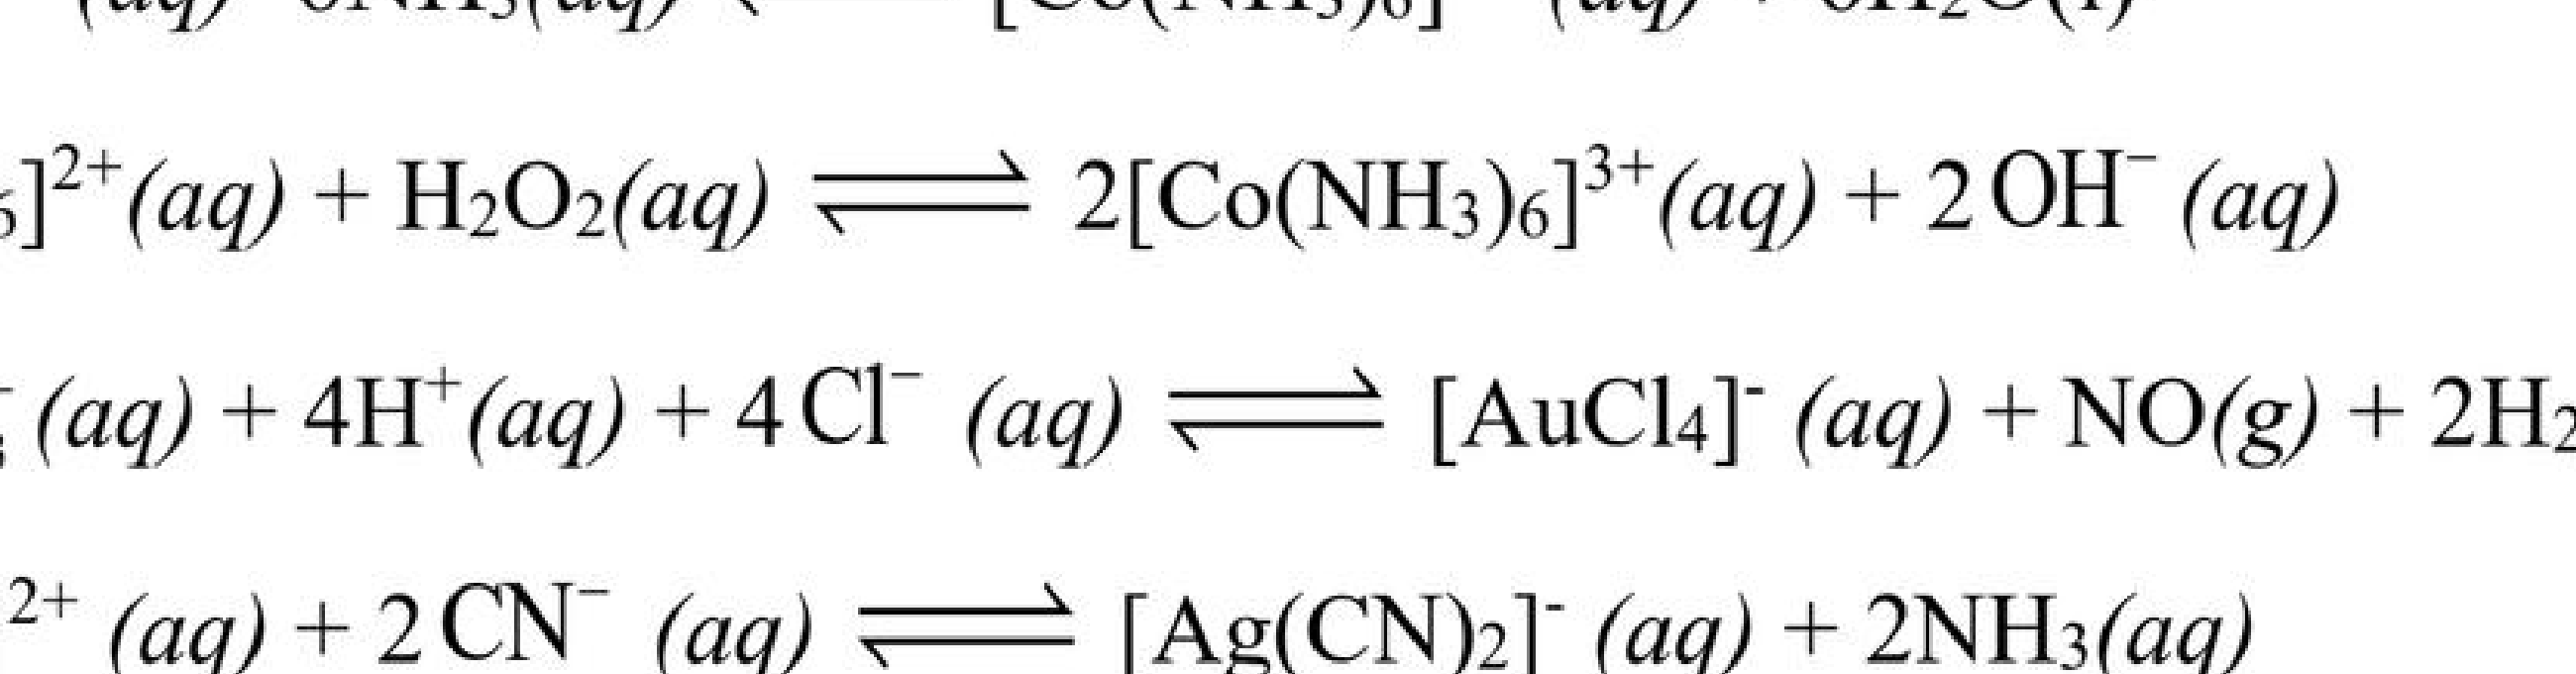
\includegraphics[height=1.4cm]{images_crop_de22/p2_cau3_cisplatin.png}}\vspace{1pt}
\choiceTF
{\True Dạng hình học của phân tử cisplatin là dạng vuông phẳng.}
{\True Nguyên tử trung tâm của phức chất cisplatin là ion $\ce{Pt^2+}$.}
{\True Trong phân tử cisplatin, các phối tử liên kết với nguyên tử trung tâm là \ce{NH3} và \ce{Cl-}.}
{\True Phân tử phức chất cisplatin có tổng cộng 4 phối tử.}
\loigiai{
Cả 4 phát biểu a, b, c, d đều \textbf{Đúng}: cisplatin có cấu trúc vuông phẳng, tâm $\ce{Pt^2+}$, liên kết với 2 phối tử \ce{NH3} và 2 phối tử \ce{Cl-} (tổng cộng 4 phối tử).}
\end{ex}

\begin{ex}
Metalloporphyrin có cấu trúc tương tự heme và được sử dụng trong y học để kiểm soát chứng tăng bilirubin máu ở trẻ sơ sinh (nguyên nhân gây vàng da ở trẻ sơ sinh). Cấu trúc của phức chất metalloporphyrin được cho như hình bên dưới:
\par\vspace{1pt}\centerline{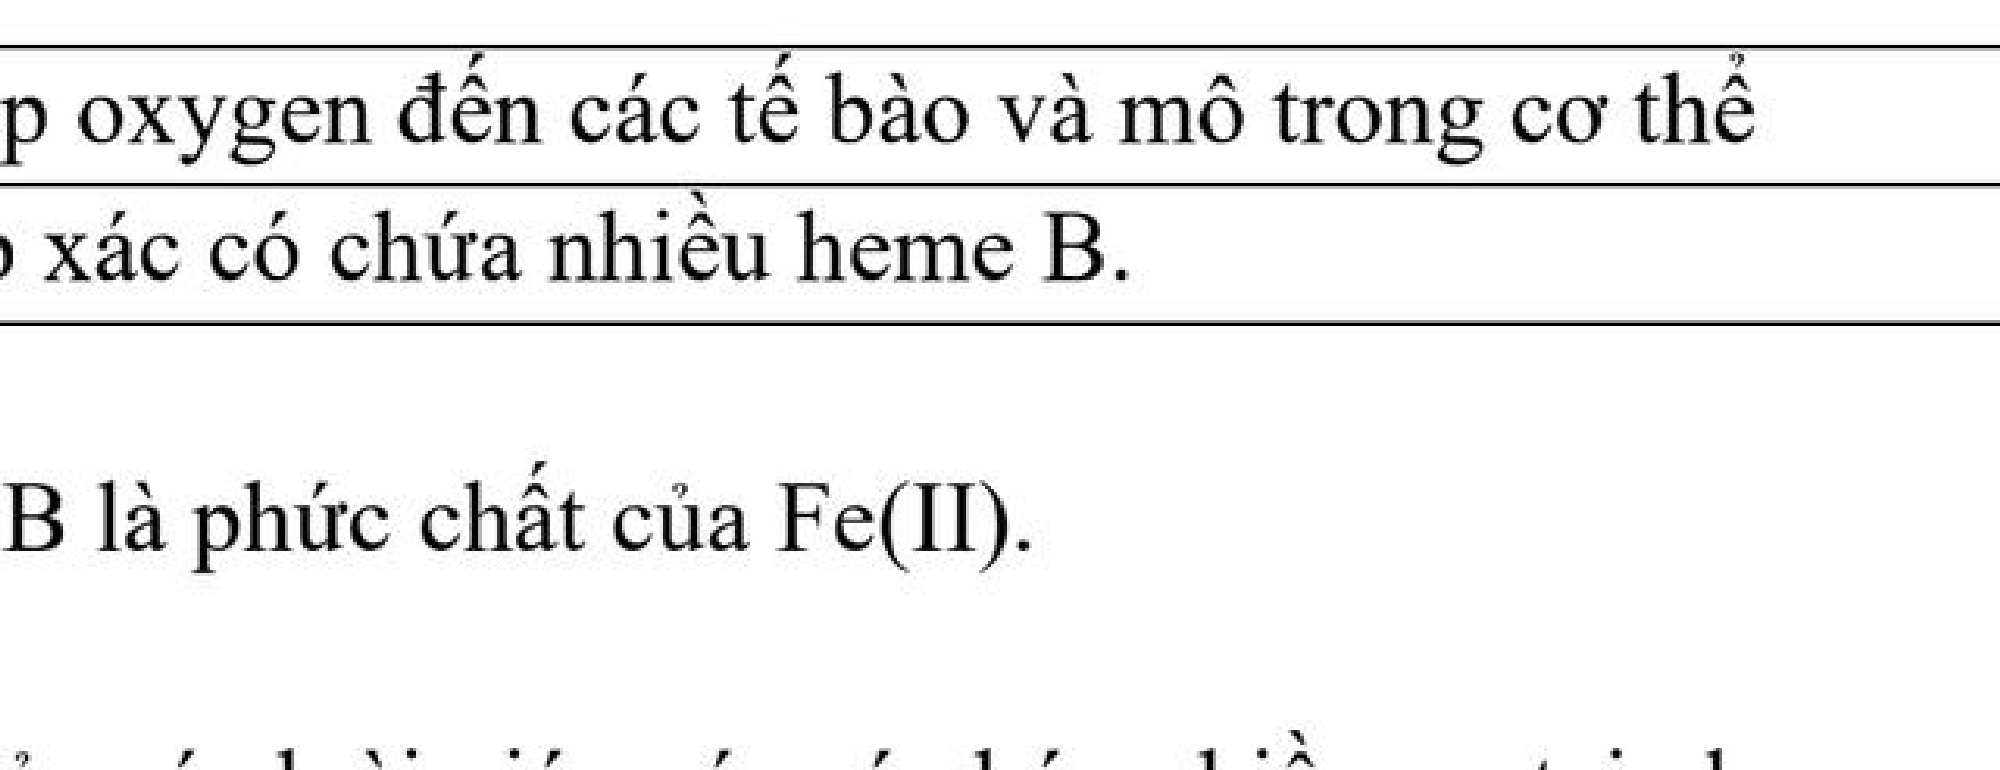
\includegraphics[height=1.5cm]{images_crop_de22/p2_cau4_metalloporphyrin.png}}\vspace{1pt}
\choiceTF
{\True Ion trung tâm của phức chất metalloporphyrin là cation $\ce{Fe^2+}$.}
{\True Số phối trí của nguyên tử trung tâm trong phức chất trên là 4.}
{Metalloporphyrin là một loại muối kép chứ không phải là phức chất.}
{\True Các liên kết phối trí trong metalloporphyrin được tạo thành do các nguyên tử N dùng cặp electron chưa liên kết cho vào orbital trống của ion $\ce{Fe^2+}$.}
\loigiai{
a) \textbf{Đúng}.\\
b) \textbf{Đúng} (4 liên kết với 4 nguyên tử N).\\
c) \textbf{Sai} vì metalloporphyrin là phức chất vòng càng chelate.\\
d) \textbf{Đúng} vì nguyên tử N cho cặp electron tự do vào orbital lai hoá trống của $\ce{Fe^2+}$.}
\end{ex}



\noindent
\textbf{PHẦN III (1,5 điểm -- 6 câu): Câu trắc nghiệm yêu cầu trả lời ngắn.}\\
\textit{Thí sinh trả lời từ câu 1 đến câu 6.}

\setcounter{ex}{0}

\begin{ex}
Cho các phức chất sau: $\ce{[Co(NH3)6]^3+}$, $\ce{[Ti(OH2)6]^3+}$, $\ce{[Zn(CN)4]^2-}$, $\ce{[Cd(CN)4]^2-}$, $\ce{[Mo(CO)6]}$. Có bao nhiêu phức chất có dạng hình học bát diện?
\par\noindent\textbf{Đáp số:} \textbf{\color{red}3}
\loigiai{
Có 3 phức chất có 6 phối tử tạo cấu trúc bát diện: $\ce{[Co(NH3)6]^3+}$, $\ce{[Ti(OH2)6]^3+}$, $\ce{[Mo(CO)6]}$.\\
\textbf{Đáp số: 3.}}
\end{ex}

\begin{ex}
Cho dung dịch \ce{NH3} đặc đến dư vào dung dịch \ce{CoCl2}, thu được dung dịch có màu hồng chuyển dần sang nâu. Hiện tượng này được giải thích là do tất cả các phối tử \ce{H2O} trong phức chất $\ce{[Co(OH2)6]^2+}$ đã được thay thế hoàn toàn bằng phối tử \ce{NH3}. Có bao nhiêu liên kết phối trí Co-N có trong phân tử phức chất mới được tạo thành?
\par\noindent\textbf{Đáp số:} \textbf{\color{red}6}
\loigiai{
$\ce{[Co(OH2)6]^2+ + 6NH3 -> [Co(NH3)6]^2+ + 6H2O}$. Có 6 phối tử \ce{NH3} tạo 6 liên kết phối trí Co-N.\\
\textbf{Đáp số: 6.}}
\end{ex}

\begin{ex}
Phức chất $\ce{[Pt(NH3)4]^2+}$ có thể bị thế bởi 1 phối tử \ce{Cl-} để tạo thành phức chất mới. Điện tích của phức chất tạo thành là bao nhiêu?
\par\noindent\textbf{Đáp số:} \textbf{\color{red}1}
\loigiai{
$\ce{[Pt(NH3)4]^2+ + Cl- -> [Pt(NH3)3Cl]+ + NH3}$. Điện tích của phức chất mới là $+1$.\\
\textbf{Đáp số: 1.}}
\end{ex}

\begin{ex}
Cisplatin là một phức chất của $\ce{Pt^2+}$ được sử dụng rộng rãi trong phác đồ điều trị ung thư. Cisplatin có thể được tổng hợp theo sơ đồ sau:
\par\vspace{1pt}\centerline{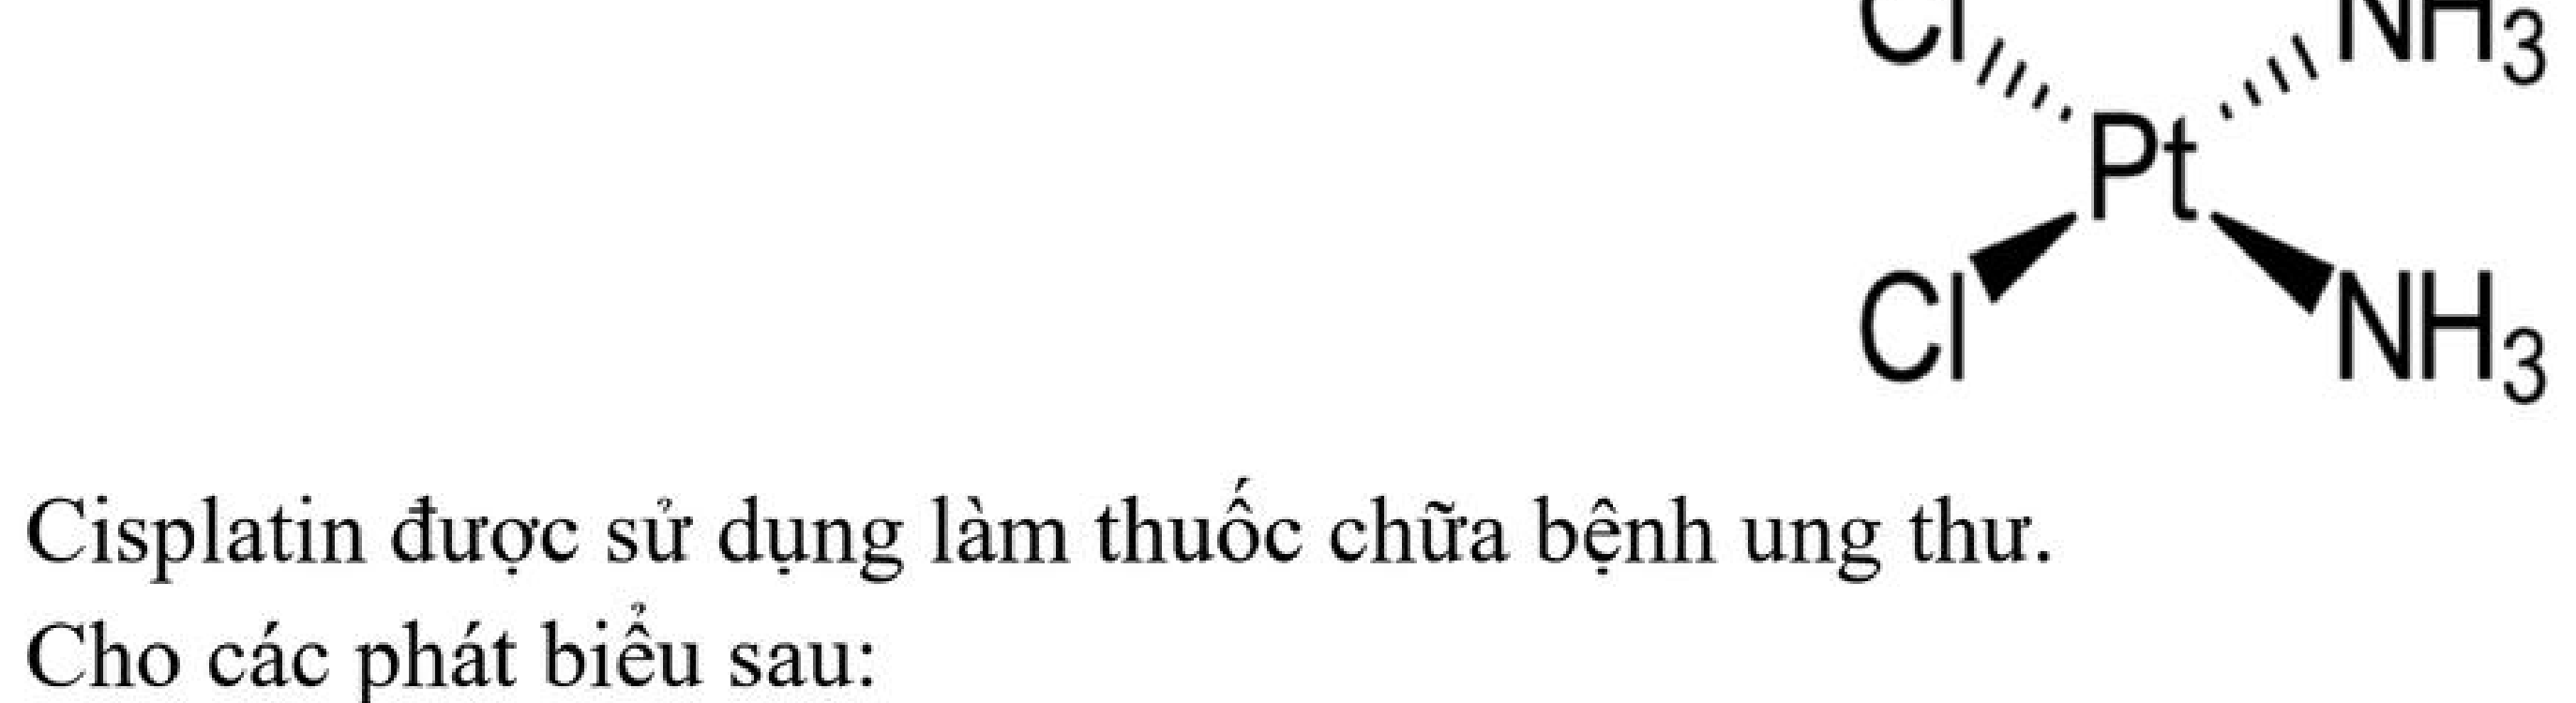
\includegraphics[height=1.35cm]{images_crop_de22/p3_cau4_so_do_cisplatin.png}}\vspace{1pt}
Xác định giá trị của điện tích $X$.
\par\noindent\textbf{Đáp số:} \textbf{\color{red}-1}
\loigiai{
Trong $\ce{[PtCl3(NH3)]^X}$: $\text{Pt}^{2+} + 3\times (-1) + 0 = -1 \rightarrow X = -1$.\\
\textbf{Đáp số: -1.}}
\end{ex}

\begin{ex}
Phức chất $\ce{[MA_{$x$}B_{$y$}]}$ có dạng hình học vuông phẳng, trong đó M là nguyên tử trung tâm; A và B là các phối tử một càng; $x$ và $y$ là số lượng phối tử của A và B. Xác định giá trị của tổng $x + y$.
\par\noindent\textbf{Đáp số:} \textbf{\color{red}4}
\loigiai{
Phức chất vuông phẳng có số phối trí bằng 4 đối với phối tử một càng $\rightarrow x + y = 4$.\\
\textbf{Đáp số: 4.}}
\end{ex}

\begin{ex}
Để tiến hành mạ đồng cho một tấm huy chương hình trụ tròn (ruột bằng sắt) có bán kính đáy $r = 2{,}5\text{ cm}$ và chiều cao $h = 0{,}3\text{ cm}$ sao cho lớp mạ đồng phủ đều mọi bề mặt với độ dày $0{,}1\text{ cm}$. Người ta tiến hành điện phân dung dịch \ce{CuSO4} 0,5 M dư với anode bằng đồng tinh khiết ở cường độ dòng điện không đổi $I = 2\text{ A}$. Biết hiệu suất điện phân là 100\%, khối lượng riêng của đồng $D = 8{,}95\text{ g/cm}^3$, lấy $\pi = 3{,}14$; $M_{\ce{Cu}} = 64\text{ g/mol}$; hằng số Faraday $F = 96485\text{ C/mol}$. Tính thời gian $t$ (theo đơn vị giờ) để hoàn thành quá trình mạ (làm tròn kết quả đến hàng phần mười).
\par\noindent\textbf{Đáp số:} \textbf{\color{red}17,7}
\loigiai{
-- Thể tích trước khi mạ: $V_1 = 3{,}14 \times (2{,}5)^2 \times 0{,}3 = 5{,}8875\text{ cm}^3$.\\
-- Kích thước sau khi mạ: bán kính mới $R = 2{,}6\text{ cm}$, chiều cao mới $H = 0{,}5\text{ cm}$.\\
$V_2 = 3{,}14 \times (2{,}6)^2 \times 0{,}5 = 10{,}6132\text{ cm}^3$.\\
-- Thể tích Cu bám vào: $V_{\ce{Cu}} = 10{,}6132 - 5{,}8875 = 4{,}7257\text{ cm}^3$.\\
-- Khối lượng Cu: $m_{\ce{Cu}} = 4{,}7257 \times 8{,}95 \approx 42{,}295\text{ g} \rightarrow n_{\ce{Cu}} \approx 0{,}66086\text{ mol}$.\\
-- $n_e = 2 n_{\ce{Cu}} \approx 1{,}32172\text{ mol} \rightarrow t = \dfrac{1{,}32172 \times 96485}{2} \approx 63763\text{ s} \approx 17{,}7\text{ h}$.\\
\textbf{Đáp số: 17,7.}}
\end{ex}

\vspace{0.3cm}
\noindent
\textbf{\color{hfRed}\large BẢNG ĐÁP ÁN THAM KHẢO TOÀN ĐỀ}

\vspace{0.1cm}
\noindent
\textbf{\color{mainGreen}PHẦN I:} 1.B \quad 2.A \quad 3.C \quad 4.C \quad 5.C \quad 6.C \quad 7.C \quad 8.B \quad 9.A \quad 10.A \quad 11.C \quad 12.C \quad 13.C \quad 14.B \quad 15.B \quad 16.B \quad 17.A \quad 18.A

\vspace{0.1cm}
\noindent
\textbf{\color{mainGreen}PHẦN II:} Câu 1: a-Đ, b-S, c-Đ, d-S \quad|\quad Câu 2: a-S, b-S, c-Đ, d-Đ\\
Câu 3: a-Đ, b-Đ, c-Đ, d-Đ \quad|\quad Câu 4: a-Đ, b-Đ, c-S, d-Đ

\vspace{0.1cm}
\noindent
\textbf{\color{mainGreen}PHẦN III:} Câu 1: \textbf{3} \quad|\quad Câu 2: \textbf{6} \quad|\quad Câu 3: \textbf{1} \quad|\quad Câu 4: \textbf{-1} \quad|\quad Câu 5: \textbf{4} \quad|\quad Câu 6: \textbf{17,7}

\Closesolutionfile{ans}
\end{document}
